\chapter{Common Diseases in Sugar beet}
\label{cha:Fundamentals}	

Disease infestations during sugar beet plantation season lead to a reduction in the quantity and quality of yields. The sections in this chapter of the paper discuss three of the most destructive sugar beet diseases. Furthermore, the causative agent, signs and symptoms, and visual representation of each disease were discussed.

\section{Cercospora Leaf Spot (CLS)}
 The causative agent of CLS - one of the most destructive foliar diseases of sugar beet- is \textit{Cercospora beticola} \cite{stewart1999phylogenetic}. This fungus attack has been reported in plantations of countries like Germany, the USA and Romania \cite{khan2005evaluating, gummert2015variety, iamandei2013biological}. CLS infection in sugar beets amounts to low-quality of extracted sugar, and a yield loss of up to 50\%  \cite{rossi2000effect}.
CLS is a leaf disease identified in infected sugar beet plants by the irregular distribution of about 2-5 mm circular leaf spots with reddish-purple margins across a mature leaf’s surface. Under humid conditions, the leaf spots become grey indicating progress in the disease development. In an advanced stage of infection, the regions damaged by the disease unite together to form a whole large group, which eventually causes the shrinking and death of the leaf. Figure \ref{fig:disease}d show a representation of a CLS infected sugar beet leaf. The spots showing the indication of CLS can be seen on the leaf surface.


\section{Powdery Mildew} 
Powdery mildew infection in sugar beet plants is characterised by the visible white/light powdery grey mould on the leaf surface. In an advanced infestation stage, the resistant cell that ensures survival from the fungus disease appears as black dots on the leaf. The causal agent is \textit{Erysiphe betae.} A plantation affected by the infestation of this fungal leaf disease can amount to a loss of approximately 30\% sugar yields \cite{francis2002sugar}.
The growth of powdery mildew disease in sugar beet is favourable in high temperature and low air humidity conditions, usually around August and October. Figure \ref{fig:disease}c show a representation of a sugar beet plant infected with powdery mildew. The figure shows a presence of white powdery mould on the leaf surface.

\section{Rhizoctonia Root and Crown Rot (RCRR)} 
The fungal pathogen \textit{Rhizoctonia solani (AG 2-2IIIB)} is a causative agent of the endemic Rhizoctonia root and crown rot disease in sugar beet cultivated in Germany and other European countries \cite{buhre2009integrated}. The harvest of a sugar beet cultivation infected with RCRR can decrease up to 80\% sucrose content due to respiration that occurs during storage if the harvested roots are not frozen \cite{campbell2014postharvest}.
% Signs and symptoms:
The foliar symptoms of Rhizoctonia root and crown rot is the dark brown lesions on the base of the petioles, which indicates wilting and loss of green colouration of the plant leaf. Figure \ref{fig:disease}a,b show a representation of an RCRR infected sugar beet leaf. The visible dark spots in figure \ref{fig:disease} b show the signs of rotting in the harvested root.


    \begin{figure}[htbp]
        \centerline{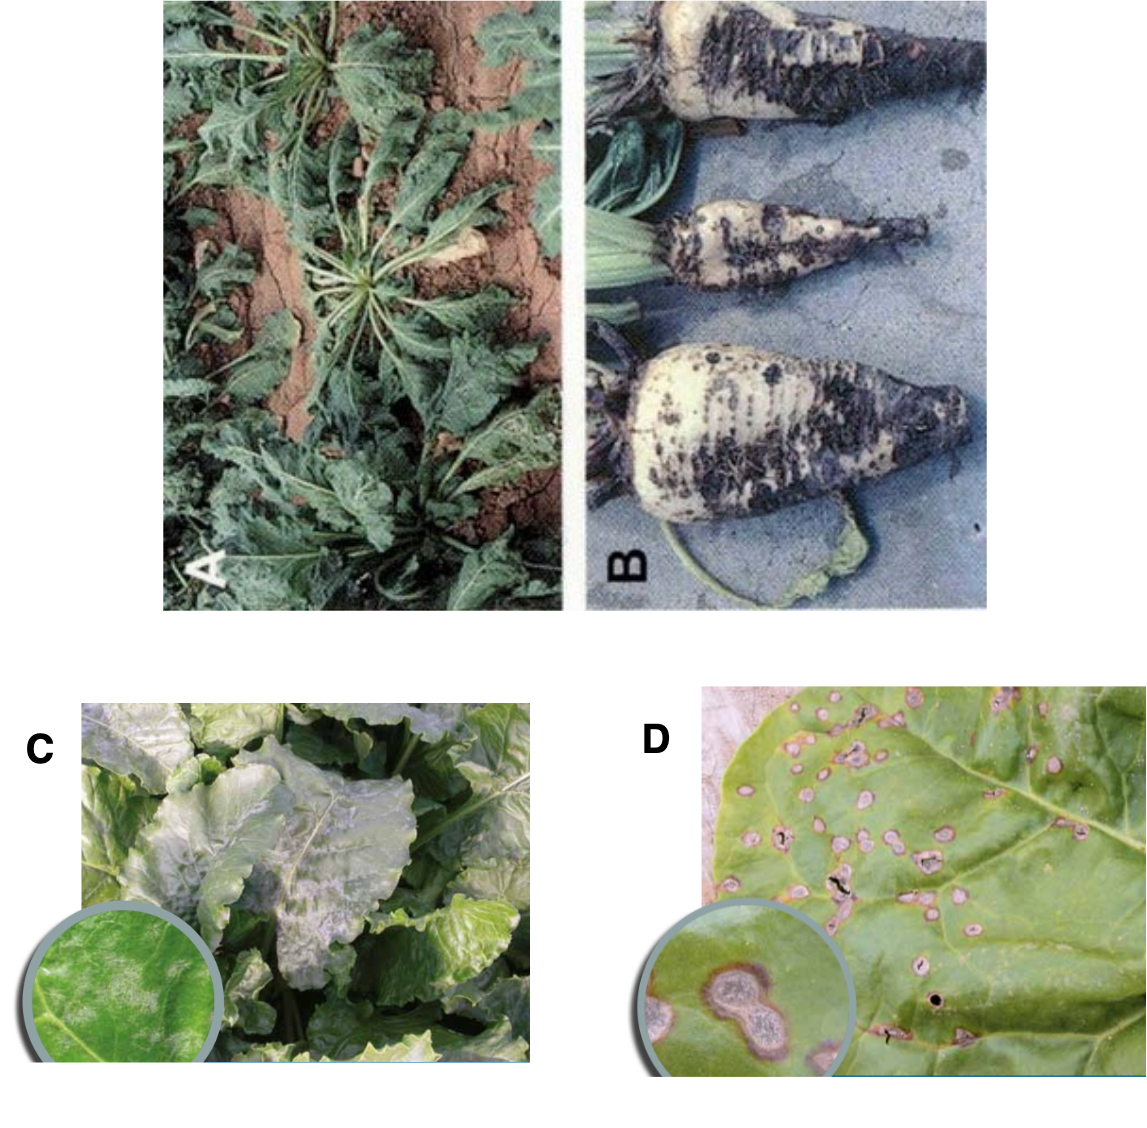
\includegraphics[scale=0.4]{figure/Untitled2.png}}
        \caption{(a,b) RCRR, (c) powdery mildew and (d) CLS disease in sugar beet \cite{articleHarveson}.}

        \label{fig:disease}
    \end{figure}

